\documentclass[11pt]{article}

\usepackage[utf8]{inputenc}
\usepackage[T1]{fontenc}
%\RequirePackage{lmodern}	% font set: Latin Modern
\RequirePackage{charter}	% font set: Charter

\usepackage[french,english]{babel}

% Package ADDED
\usepackage{xcolor,graphics,graphicx}

% For citations
\usepackage{csquotes}

% For line spacing
\usepackage{setspace}
\linespread{1.3}

% To rotate a table or a figure
\usepackage{lscape}

% To manage cells in table
\newcommand{\tabcell}[2][c]{%
	\begin{tabular}[#1]{@{}l@{}}#2\end{tabular}}

% MATHS
%% The amssymb package provides various useful mathematical symbols
\usepackage{amssymb}
\usepackage{amsmath}
\usepackage{empheq}

% TAILLE de la page
\usepackage{geometry} % define page margin
\geometry{top=20mm,left=20mm,right=30mm,bottom=20mm} % margin from top, left, right and bottom

% COMPTEUR de ligne
%% The lineno packages adds line numbers. Start line numbering with
%% \begin{linenumbers}, end it with \end{linenumbers}. Or switch it on
%% for the whole article with \linenumbers after \end{frontmatter}.
\usepackage{caption}
\usepackage{lineno}
\linenumbers

% BIBLIOGRAPHIE
%\usepackage[numbers]{natbib}
\usepackage[authoryear]{natbib}
\usepackage{hyperref}

\begin{document}

\begin{center}
	\Large\textbf{
	Trophic transfer of anticoagulant rodenticides while managing rodent pests: the fine line between predator-prey regulation and pesticide-pest regulation
}\par
\end{center}

\vspace{.5cm}

\begin{center}
	\large\textbf{
		Virgile Baudrot$^{1,2}$ 
		Javier Fernandez-de-Simon$^{1,3}$
		Michael Coeurdassier$^1$,
		Geoffroy Couval$^{1,4}$,
		Patrick Giraudoux$^1$,
		Xavier Lambin$^{5,6}$		
	}\par	
\end{center}
~\\
$^1$ Université Bourgogne Franche-Comté - UMR CNRS 6249 Laboratoire Chrono-environnement, 25030 Besançon, France\\
$^2$ BioSP, INRA, 84000 Avignon, France\\
$^3$ IREC. Instituto de Investigación en Recursos Cinegéticos\\
$^4$ FREDON Franche-Comté, Espace Valentin Est, 12, Rue de Franche-Comté - Bât E, 25480 Ecole-Valentin, France\\
$^5$ School of Biological Sciences, University of Aberdeen, Zoology Building, Tillydrone Avenue, Aberdeen AB24 2TZ, Scotland, UK\\
~\\
$^*$ Corresponding authors: \textcolor{gray}{virgile.baudrot@posteo.net or x.lambin@abdn.ac.uk}

\paragraph{Running Title} \textcolor{gray}{Bufferscapes to preserve Non-Target Organism / Ecosystem services}

\vspace{.5cm}

\begin{abstract} ~
	\begin{enumerate}
		\item Understanding pesticide impacts on populations of target/non-target species and communities is a challenge to applied ecology. When predators that otherwise regulate pest densities ingest prey contaminated with pesticides, this can suppress predator populations as contaminated prey act as a super-predator, with pesticides controlling both pest and predators. It is, however, unknown how species relationships and protocols of rodenticide treatments, i.e. farmer functional responses, interact to affect pest regulation.
		\item Here we used linked differential equations to model a heuristic non-spatialized system including montane water voles, specialist vole predators (stoats, weasels), and a generalist predator (red fox) which consume voles, mustelids and other prey. By considering anticoagulant rodenticide toxicokinetic and toxicodynamic equations, we explored the impact of 5 farmer functional responses (defined by both rodenticide quantity and threshold vole density above which rodenticide spreading is prohibited) on predator-prey interactions, rodenticide transfer across the trophic chain and population effects.
		\item Spreading rodenticide while maintaining sufficient voles as prey resources led to less rodenticide being applied and extended periods without rodenticide in the environment, benefitting predators while avoiding episodes with high vole density. This may meet farm production interests while minimizing the impact on small mustelid and fox populations.
		Spreading rodenticide to maintain low vole densities suppressed mustelid and fox populations, leading to vole population dynamics being entirely regulated by rodenticide use. This vole-eradication treatment regime inhibited predator ecosystem services and promoted pesticide dependence.
		\item Farmer functional response with high or intermediate densities thresholds triggering treatment produced vole population fluctuations caused by rodenticide that could be followed by periods during which mustelids regulated vole populations. These alternative phases of mustelids and farmer regulation highlight the benefit of intraguild relationship where mustelids may rescue foxes from poisoning.
	\end{enumerate}

\paragraph{Synthesis and applications} Different farmer functional responses lead to a rich variety of population dynamics in predator-prey systems. That such a pesticide-tri-trophic system may cause a variety of population dynamics responses to pesticide use in agro-ecosystems is a novel insight. Our model reveals the need for maintaining refuges with sufficient non-poisoned voles for specialist mustelids, to conserve predator community, given the super-predator role of rodenticides. We suggest that long periods without pesticide treatment are essential to maintain predator populations, and that practices of pesticides use that attempt to permanently eradicate a pest over a large scale are counterproductive. 

\end{abstract}

\paragraph{Keywords} Biodiversity conservation; bromadiolone transfer; cyclic fluctuations; pesticides impact; secondary poisoning; super-predation; cascade effects

\section{Introduction}

Since the “green revolution” following the 1950s, pesticides use has increased to control pests damaging properties, public health or crops \citep{Tilman2002}. Pesticides usage is varyingly triggered by the perception/estimation of pest densities. Natural enemies (e.g., predators, parasites, competitors) also reduce pest densities and hence may preclude the need for using pesticides \citep{Michalko2017}. Natural enemies are, however, also affected by pesticides, either by direct exposure, through ingestion of contaminated prey \citep{Berny2007} or indirectly by cascade effects of resource depletion \citep{Halstead2014}.  Thus, under some regimes of pesticides use, pest populations only become regulated by pesticides once predators have collapsed. To preserve ecosystem health and the services of predators through regulation of pest densities, we need to assess the feasibility and benefit of pesticide treatment regimes in their ability to control pest species with minimal damage on predators \citep{Halstead2014}. It is however empirically challenging to assess the overall impact of pesticide treatments on the dynamics of species linked by trophic interactions. In this context, process-based models describing simplified scenarios are powerful tools to reveal hidden patterns by disentangling processes emerging from pesticide impacts on predator-prey system (e.g., \citet{Baudrot2018}).

Voles and other grassland rodent species undergo multi-annual population cycles (e.g.,  \cite{Krebs2013}. At their peaks, they may attain extremely high densities, causing substantial damage to grass/cultivated crops and forestry and conflicts with humans \citep{Delattre2009}. Farmers worldwide expand financial resources to purchase and spread anticoagulant rodenticides (hereafter AR), hoping to reduce vole populations and damages and increase profits despite the investment required \citep{Stenseth2003}. They do so according to protocols, equivalent to farmer functional responses (hereafter FFR), that involve varying amounts of AR spread in response to different thresholds in vole densities. 

Voles and many small rodents are perceived as pests, but they are also keystone species, crucial to the functioning of grassland ecosystems, as well as being the prey of numerous predators, including species of conservation concern \citep{Delibes-Mateos2011, Coeurdassier2014}. Their population cycles create pulses of resources crucial to the viability of a wide range of resident predators and the aggregation of mobile avian vole predators \citep{Korpimaki1991}. The smallest mustelids (e.g. weasels Mustela nivalis) are specialist vole predators. Their numerical response has been shown theoretically to be necessary for generating predator-prey cycles \citep{Hanski1991}. They are said to be responsible for driving 3-to-5-year vole cycles in Fennoscandia (specialist predation hypothesis) \citet{Hanski1991}. Generalist resident predators like foxes (Vulpes vulpes) are expected to have regulatory and limiting effects on voles, owing to dietary plasticity that slows down vole population increase at low density \citet{Hanski1991}. Foxes do not show numerical responses to vole abundance \citep{Weber2002} but they influence the food chain through occasional killing and consumption of bite-sized mustelids. Mustelids form a small proportion of fox diet (0-10\%) but their offtake could represent a significant portion of the population (reviewed in \citet{Lambin2018}).

Anticoagulant rodenticides are non-selective toxicants with deleterious effects on non-target fauna (e.g. \cite{Coeurdassier2014}. Despite AR being exclusively licensed for rodent control, a large number of predator species are secondarily exposed to AR \citep{Sanchez-Barbudo2012}. Repeated consumption of dead and sub-lethally intoxicated voles reduced fox abundance in farmland in eastern France \citep{Jacquot2013} and ARs caused short-term declines in stoats in New Zealand \citep{Alterio1996}. Rodent-eating mustelid populations are affected by ARs given the pervasive levels of contamination reported \citep{McDonald1998}. Thus, there is little doubt ARs use inadvertently depresses predator populations. As they likely limit vole populations, it is essential to understand when AR use becomes counterproductive by altering the pest population dynamics, producing more frequent outbreaks and high residual vole abundance.

With the aim of understanding the potentially complex interactions between prey that are perceived as pest predators and farmers spreading rodenticide in response to vole abundance and their functional responses, we studied a simplified system inspired by cyclically fluctuating montane water voles (\textit{Arvicola scherman}), small mustelids (stoats, weasels) that mostly eat voles (specialists), and foxes (generalists), with voles and mustelids as food items. We used a process-based model using differential equations to explore 5 FFR types of AR spread, combining population dynamics, predator-prey interactions and rodenticide transfer across the trophic chains. Model parameters and FFR were inspired by farming systems in the Jura Mountains, Franche-Comté (France), the region of Comté cheese production. In Franche-Comté, farmers shifted from polyculture to almost exclusively grass production for milk used to produce cheese from the early 1970s \citep{Giraudoux1997}. Due to recurrent vole outbreaks and damages to grasslands, massive rodenticide treatments were implemented from the early 80s with consequences on non-target wildlife. Practices developed technically under pressure from public opinion, farmer unions and farmer technical organizations collaborating with researchers to find treatment regimes with less harmful consequences for biodiversity \citep{Delattre2009}. 

Hence, our main objective was to explore the properties of FFR in relation to varying vole density, to vole outbreak frequencies, to the guild of interacting predators and the effects on the global tri-trophic population dynamics. Additionally, we sought to establish under what regime of use the ARs deliver benefits to farmers without imposing damages to the ecosystem. 

\section{Methods}

We specified and parameterized the tri-trophic system of voles-mustelids-foxes with use of AR by farmers in response to vole density. We considered different FFR to assess AR upward transfer through the trophic web, considering the coupled dynamics of pulsed of AR spread and population dynamics. In all cases, parameterization units are on hectare$^{-1}$ and day$^{-1}$.

\subsection{Model for the tri-trophic dynamic}

We considered a tri-trophic system described by Figure~\ref{fig:scheme} and equations (1-5); parameterization is provided in Table~\ref{tab:parameterization}. Voles, denoted $V$, were the primary prey, Mustelids, $M$, intermediate predators, and Foxes, $F$, were top predators, consuming voles and mustelids. For each species, the instantaneous variation of population size over time is:

\begin{equation}
\left\{
\begin{array}{l l}
\dfrac{dV}{dt} & = V r_V \left( 1- \dfrac{V}{K_V}\right) - \Phi_{V,M}(V)M - \Phi_{V,F}(V,M)F\\[.3cm]
%
\dfrac{dM}{dt} & = \varepsilon_M \Phi_{V,M}(V)M - m_M M - \Phi_{M,F}(V,M)F\\[.3cm]
%
\dfrac{dF}{dt} & = F r_F \left( 1- \dfrac{F}{K_F}\right)
\end{array}
\right.
\end{equation}

The vole population followed a logistic growth rate, with $r_V$  the maximal reproduction rate, fixed at $r_V = \ln(2 \times 600)/365$ per day, since montane water vole populations can increase from 0  to  600 individuals ha$^{-1}$ or more \citep{Giraudoux1997} resulting in the equilibrium density being fixed at $K_V = 600$ individuals. 
%
The vole population was preyed upon by mustelid and fox populations. The vole consumption rate at different vole densities was described by functional responses ($\Phi_{V,M}$ for mustelids, $\Phi_{V,F}$  for foxes), see equations \eqref{eq:functionResponse}.
%
We treated small mustelids as vole specialist predators \citep{King2006}, assuming a Holling Type 2 functional response with attack rate $a_M$ and handling time $h_M$ (equation \eqref{eq:functionResponse}). We then represented foxes feeding on voles and mustelids by a multi-species functional response derived from Holling Type 3, referring to generalist feeding behaviour \citep{Baudrot2016}. For that, we denoted $a_{VF}$ and $a_{MF}$ the fox attack rate on voles and mustelids respectively. The parameter $h_F$ was the handling time for foxes.


\begin{equation}
\begin{array}{l l}
 \Phi_{V,M}(V)M = \dfrac{a_M V}{1 + h_M a_M V} \\[.3cm]
 %
 \Phi_{V,F} = \dfrac{a_{VF} V}{a_{VF}V + a_{MF}F} \times \dfrac{(a_{VF}V + a_{MF} M)^2}{1 + h_F(a_{VF}V + a_{MF} M)^2}\\[.3cm]
 %
  \Phi_{M,F}(V,M)F = \dfrac{a_{MF}V}{a_{VF}V + a_{MF}F} \times \dfrac{(a_{VF}V + a_{MF}M)^2}{1+h_F(a_{VF}V + a_{MF}M)^2}
\end{array}
\label{eq:functionResponse}
\end{equation}

Parameterization of functional responses was estimated to fit the daily satiation level of predators for handling times, and the observed 5-6 year vole cycles for attack rates (Table~\ref{tab:parameterization}). We assumed foxes spent longer searching for voles than mustelids, based on each species diet and daily number of individuals captured. Therefore, $a_{VF}$ was considered larger than $a_{MF}$ and selected to produce 6-year vole cycles without AR.


Since we assumed small mustelids behave as specialist predators, we considered a numerical response linearly dependent on the functional response with parameter $\varepsilon_M$ (dimensionless) as conversion efficiency of prey into newborn predator (Supporting Information). The mustelid background mortality rate (i.e. all other reasons of death: ageing, disease, etc.) was $m_M$ parameterized has the inverse of life expectancy (Table~\ref{tab:parameterization}). 
We assumed foxes had a logistic growth rate function, parameterized with maximal growth rate $r_F = ln(3)/365$ and equilibrium density $K_F = 0.03$ [individuals.ha$^{-1}$] \citep{Ruette2003} without numerical response \citep{Weber2002}. 

\subsection{Model with rodenticide}

Figure~\ref{fig:scheme} represents the whole study system. Rodenticide is spread in grasslands during treatments, denoted $T_{Broma}(V)$, triggered by vole density $V$ (FFR described in Table~\ref{tab:results}).
%
Firstly, baits (50 mg kg$^{-1}$  of bromadiolone, hereafter AR) were spread in grasslands at quantity 7.5 to 20 kg ha$^{-1}$ day$^{-1}$. Notation day$^{-1}$ stands because of the daily time resolution.
%
Such quantity, $C$, was available for voles, and a proportion disappeared in the environment at rate $k_0$ (set at $k_0 = 0.0815$) \citep{Sage2008}. The proportion consumed per vole, with rate $\kappa(C)$, was assumed to be an increasing function. The function $\kappa(C)$ was characterized by a maximum ingestion $M_{in}$, and a half-saturation constant for ingestion $D_{in}$ in [mg kg$^{-1}$]:

\begin{equation}
\kappa(C)= \dfrac{M_{in}\times C}{D_{in} + C}
\end{equation}

For the toxicokinetics of AR (i.e. internal compound dynamics) leading to AR concentrations in animal body (voles, mustelids and foxes), we considered an uptake without biotransformation and time-regulated distribution, (i.e. AR concentration in the body of animals was instantly homogeneous) and that the whole body was consumed or scavenged without selection/rejection of tissues-organs. We also assumed disappearance including excretion of the parent compound and metabolisation, and that metabolites were non-toxic and/or excreted in the scats. 
For the toxicokinetics of AR ingested by voles, a fraction $C_V$ was assumed to remain active, stored mainly in vole livers and available to predators ingesting voles. The absorption rate of ARs ($\eta$) exceeds 50\% in less than 24h \citep{Jacquot2013}. The excretion rate from voles, $k_{out}$, $V$ was 0.4 day$^{-1}$ \citep{Sage2008}. The mortality rate through ARs was $\mu(C_V)$. Death through poisoning created a dead vole population ($V_d$) with AR concentration $C_V$. Dead voles could either be scavenged by mustelids/foxes or decompose at rate $d$. We assumed AR in dead voles disappeared from the system when voles decomposed. 
Mustelids could feed on live voles $V$, or non-decomposed dead voles Vd and we assumed a Type 2 functional response adapted for a multi-species functional response \citep{Baudrot2016}. Mustelids ingested AR with absorption rate $\eta_M$ (ratio between biomasses of voles, $B_V$, and mustelids, $B_M$) and the total of ingested voles (alive $V$ and dead $V_d$) was defined by function $\Theta_M (V,V_d=$ (Table~\ref{tab:parameterization}).

A fraction of AR ingested was accumulated in weasels while the rest was excreted with rate $k_{out,M}$.
%
AR provided to weasel though vole poisoning, is denoted $D_M$ induces lethal effect at rate $\mu_M(D_M)$, additive to natural mortality rate $m_M$. Parameter definition are further detailed in Supporting Information.
%
AR was ingested by foxes with a rate proportional to the functional response of foxes to voles, dead voles and mustelids.
%
Foxes also accumulated AR available in their prey, resulting in upward AR transfer in the trophic chain. Foxes accumulated AR in concentration $C_F$. A fraction of AR was excreted by foxes at rate $k_{out,F}$ at a rate between 0.38 and 0.72 [day$^{-1}$]\citep{Sage2010}, and AR caused fox mortality at rate $\mu_F$ ($D_F$).

We used log-logistic equations for describing dose-dependent mortality of animals exposed to AR. Vole and predator mortality rates due to AR $\mu_X(\zeta_X)$ ($X$ referring to the considered species, and $\zeta_X$ being the dose eaten $D_X$ or the internal concentration $D_X$) were expressed by equation (5):

\begin{equation}
\mu_X(\zeta_X) = \dfrac{1}{\text{experiment duration}} \times \left( 1- \dfrac{1}{1+ (LD_{50}/\zeta_X)^H} \right) 
\label{eq:muX}
\end{equation}

where $LD_{50}$ was the daily median lethal dose (50\% of population dying) with a value for voles of 2 mg kg$^{-1}$ as internal concentration, and a dose given as food of  2.1 mg kg$^{-1}$ mustelids \citep{Grolleau1989} and 0.5 mg kg$^{-1}$ for foxes \citep{Sage2010} (see Table~\ref{tab:parameterization}). Parameter $H$ is the Hill's coefficient, modulating the curve steepness and was estimated to fit the sparse data we have (Table~\ref{tab:parameterization}). Mortality rates considered the duration of AR toxicity from experiments of up to 6 days \citep{Sage2010}.

\subsection{The farmer functional responses explored through simulation}

We considered a range of realistic FFR spanning treatments during vole outbreaks only as a precautionary approach; in which treatments only takes place at intermediate or low vole density threshold. These scenarios are inspired by historic and contemporary protocols of bromadiolone use to control montane water voles in Franche-Comté, but also representative of practice globally (Table~\ref{tab:results}) \citep{Delattre2009}. To check the influence of foxes and intraguild predation on the system’s dynamics, we simulated scenarios with and without foxes.

Our simulations tracked the linked vole-mustelid-fox dynamics for 40 years, after a “burn-in” period of 10 years to reduce dependency of results upon initial conditions, to observe several vole cycles and to characterise AR effects on these species population dynamics. This burn-in period also had AR treatment triggered at specific vole densities and with a given rodenticide quantity for each FFR (see Table~\ref{tab:results}). The burn-in phase was selected according to a set of simulations with different initial conditions. Those simulations showed that in a given FFR (i.e., same threshold of vole density and amount of AR spread), the dynamics of the population were converging toward a similar pattern. 
In order to assess the impact of FFR on both agriculture and conservation interests, we estimated the following cost functions: (i) Number of treatment events per FFR ; (ii) Cumulative amount of AR (kg) ; (iii) Proportion of time when the AR-induced mortality of mustelids higher than 50\% (i.e. lethal exposure profile killing 50\% of mustelid population) ; (iv) Proportion of time when the mortality of mustelids was higher than 50\% due to natural mortality; (v) Proportion of time when the vole density was below 50 voles ha$^{-1}$, as a proxy for time when forage grass grows with low herbivore influence; (vi) Mean vole, mustelid and fox densities.

\subsection{Numerical Simulation and Sensitivity Analysis}

All numerical analysis have been done using the Open language R and particularly the ODE solver package \textit{deSolve} \citep{Soetaert2010}. Model implementation and code to run analysis are available on the Github repository \url{https://github.com/virgile-baudrot/trophToxNTO/}.
%
From simulations, a sensitivity analysis allowed to study \textit{how uncertainties in the model output are apportioned to different sources of uncertainty in the model input} \citep{Saltelli2019}.
%
We applied a global approach using the first-order Sobol's sensitivity index $S_i$ defined as $S_i = \mathbb{V}(\mathbb{E}_{-i}(y \vert x_i)) / \mathbb{V}(y)$, where $\mathbb{V}(y)$ is the variance of $y$ when all factors are allowed to vary, $\mathbb{E}_{x\sim i}(y \vert x_i))$ the mean of $y$ when one factor is fixed \citep{Sobol1993}. We defined the domain of variation with a beta distribution within an hyperspace of plus or minus 10\% from the original value for all parameters.

\section{Results}

\subsection{Population dynamics}

Allowing for mortality by predators ingesting AR-poisoned voles changed the outcome of predator-prey dynamics involving vole, mustelid and fox populations. Secondary poisoning led to a rich spectrum of emergent dynamics according to the FFR to vole abundance.  
Without AR (FFR a), vole dynamics were regulated by mustelid predation that gave rise to 6-year cycles (Figure~\ref{fig:populations}). The fox population remained at its carrying capacity (i.e., 0.03 ind ha$^{-1}$, see Table~\ref{tab:parameterization}).  

Under FFR b (high vole density threshold triggering treatment and high AR amount per treatment) and FFR d (intermediate threshold and low AR amount), vole dynamics were sequentially regulated by either AR treatments, which we refer to as farmer-regulated phase (red color sections in Figure~\ref{fig:populations}), or by mustelids, mustelids-regulated phase (blue color sections in Figure~\ref{fig:populations}). Farmer-regulated periods started when densities of living voles triggered treatments. This produced sudden declines of live voles followed by increases of dead voles. However, the vole population re-grew quickly which triggered frequent further treatments and pulses of availability of contaminated (both live and dead) voles. In FFR d (intermediate threshold and low AR), vole declines were not as deep as when pulses of AR amount were high (FFR b), owing to the reduced rodenticide amount per treatment. Mustelids and foxes also experienced AR-induced declines during this period. Under FFRs b (high threshold density, high AR) and d (intermediate threshold, low AR), mustelid-regulated periods started when mustelid numbers grew slowly to a peak, which depressed vole density, precluding rodenticide treatments and releasing the fox population from secondary poisoning, such that its abundance rebounded. Vole depletion by mustelids and subsequent mustelid declines allowed the vole population to grow again up to threshold densities and initiated a new period of regulation by farmers.
%
Vole dynamics were permanently regulated by AR treatment under FFR c (intermediate threshold, high AR, Figure~\ref{fig:populations}-c). Populations of live and dead voles experienced high frequency fluctuations (around 2 peaks every year) driven by AR. As AR treatments were frequent, being triggered by voles peaks, contaminated dead voles were always abundant (peaks at 90 ind ha$^{-1}$), and mustelid and fox densities remained low (see Supporting Information: mustelids <0.150 ind ha$^{-1}$ and foxes <0.01 ind ha$^{-1}$) but with a slowly increasing trend on the long term period (Figure~\ref{fig:populations}-c). This pattern of an increasing trend appears to be very sensitive to parameterization (i.e. a slight change in parameter may lead to a long-term decreasing pattern).
%
With FFR e (low threshold, low AR), vole populations were maintained by farmers at around 50 voles ha$^{-1}$ (See Figure~\ref{fig:populations} and Supporting Information). The population of live voles was buffered by treatments. Additionally, whenever voles reached densities triggering treatment, predator populations experienced strong declines. However, fox densities were higher compared to FFR c (intermediate threshold, high AR) (>0.01 ind ha$^{-1}$, see Supporting Information), reflecting the reduced amount of AR used (7.5 kg) and transferred to foxes as there were lower vole densities. The maximum numbers of dead voles under this FFR e was relatively low (highest around 15 ind ha$^{-1}$) but, due to frequent treatments, there was a steady replenishment of contaminated dead voles. This, in turn, induced mustelid and fox mortality and population declines (Supporting Information). Additionally, low availability of live voles triggered small mustelids mortality through starvation down to abundances similar to those resulting from AR use (Supporting Information). 

\subsection{Comparison between farmer functional responses in terms of cost functions}

As expected, spreading AR generally reduced vole densities (Table~\ref{tab:results}) but the extent to which it also affected predators and the costs and benefits for conservation and farmer’s interests varied widely. 
The FFR b (high threshold, high AR) and d (intermediate threshold, low AR) implied the lowest number of treatments (0.5 and 1.8 year$^{-1}$ respectively) and the lowest amount of AR used (mean 10 and 13.5 kg ha$^{-1}$ year$^{-1}$ resp.). The FFR e (low threshold, low AR) had the lowest mustelid mortality due to AR (no instance in 40 years) but maximised starvation-induced mortality of mustelids (Table~\ref{tab:results}). Additionally, FFR e (low threshold, low AR) had the highest proportion of time with < 50 voles' ind ha$^{-1}$, (91\% of study period). When considering the effectiveness in reducing mean vole densities over the long-term period, FFR e (low threshold, low AR) ranked highest (only 55 ind ha$^{-1}$ in means, and >118 ind ha$^{-1}$ for other scenarios). The FFR b (high threshold, high AR) and d (intermediate threshold, low AR) allowed the highest mean densities of mustelids and foxes.
%
Comparison of these protocols indicates that FFR b and d, inducing successive farmer-regulated and predator-regulated phases, were the best scenarios for conservation interests (Table~\ref{tab:results}).

\subsection{Influence of intra-guild predation}

Figure~\ref{fig:intraguild} shows the system dynamics under FFR d, where successive farmer-regulated and mustelids-regulated phases occured. This simulation shows that the removal of foxes did not eliminate the successions of mustelids-regulated and farmer-regulated phases. However, the mustelid regulated period allowed short-term peaks of voles, suggesting the emergence of a classical one-predator - one-prey cycles interrupted by a farmer-regulated period. Without foxes, population dynamics of mustelids presented a more chaotic behaviour, while it presented regular cyclic pattern with fox occurrence. Therefore, this simple model suggests a stabilizing role of a generalist predator (foxes in this system) during the mustelid-regulated period. At the end of the mustelid-regulated period, foxes strongly contributed to vole mortality and, to a lesser degree, mustelid mortality. Consequently, the removal of foxes implied less predation over voles during the mustelid regulated period, and short-term vole releases from mustelid predation. The 2-year rolling mean of vole density (blue lines in Figure~\ref{fig:intraguild}) illustrates the change of regime from farmer-regulated to mustelids-regulated phases. Indeed, the amplitude of averaged vole densities (i.e., the amplitude of vole cycles for the 2-year rolling mean) was relatively stable at the beginning of farmer regulation period and then suddenly decreased to become minimal before sharply increasing, announcing the regime change. These changes in density amplitude may be used as an early-warning signal of the regime transition. 

\subsection{Sensitivity of model under this parameterization}

%
Figure~\ref{fig:sobol_sensitivity} represents the global sensitivity where we computed a first order sensitivity index \citep{Sobol1993, Saltelli2019} given the contribution of each parameter to the variance of the model d (i.e., 7.5kg of AR at threshold density of 250 voles).
%
Parameters are moved within +/- 10\% interval around the fixed value as defined in scenario d (see Table~\ref{tab:parameterization}).
%
Crossing all cost functions to test the sensitivity of model parameters, the influence of each parameter appears quite homogeneous.
%
There is no redundant or conversely any parameters with a dominant influence on model behaviour.
%
Taking cost functions separately, the sensitivity to parameters present some differences.
%
This is particularly true for densities of predators on which we focus our attention.  
For mustelids and foxes variable.

% For instance, the vole carrying capacity $K_V$ has a strong influence on density of predators and the number of treatments, but few on the vole density (i.e., mean vole density and period of time with less than 50 vole/ha) reflecting the fact that vole population is totally regulated by predation (i.e., density of predators) or poisoning (i.e. number of treatment) but not by resource of voles.
%
% On the contrary, lethal dose for 50\% of mustelids, $LD_{50,M}$, has a strong influence on mean vole density and is weaker for other cost functions.
%
% From the sensitivity analysis, the drivers of the mean density of mustelids are the mustelids' resources, which is the carrying capacity of vole, $K_V$, and the parameters reflecting intrinsic mustelids parameter as the natural mortality rate $m_M$, and toxicological parameters of mustelids as the Hill's coefficient, the lethal dose for 50\%, and those of voles as the half saturation intake rate of contaminant for voles $D_{in}$ and the vole excretion rate of AR, denoted $k_{out,V}$.


\section{Discussion} 

Considering that rodenticide kills not only voles but also their predators through secondary poisoning, our models show that AR profoundly changes the outcome of predator-prey dynamics involving vole, mustelid and fox populations beyond what mere intuition could elucidate. Our study reveals how the dual influences of the amount of pesticide spread and the vole density threshold triggering AR spread drives (i) pesticide spreading frequency, (ii) predation ecosystem service, and subsequently (iii) the control of pest outbreaks. Two types of a rich spectrum of emergent dynamics, including farmer or mustelid regulation deviating from classical predator prey dynamics arose because poisoned voles acted as “super-predators”. 

\subsection{Modelling farmer regulation into a classical predator-prey system}
 
The threshold functional response of farmers deciding when to apply varying amounts of rodenticides according to prevailing vole density was crucial in selecting the emergent ecosystem dynamics, resulting in much variability in ecosystem and conservation and farming production interests. In the ecosystem our models depict, farmers spreading rodenticide not only depleted vole prey exploited by specialist and generalist predators but also created pulses of lethally or sub-lethally poisoned voles that became super-predators by poisoning their predators.  Arguably this set of ecological interactions has similarities with circumstances where a pathogen affecting prey species also infects predators, as in the case with the flea vectored plague (\textit{Yersinia pestis}) infecting prairie dogs (\textit{Cynomys} spp.) and black footed ferrets (\textit{Mustela nigripes}) in central US \citep{Matchett2010}. However, to our knowledge, the behaviour of such tri-trophic model with multiple reciprocal interactions has not been explored. This is despite the obvious relevance to the management of the globally widespread circumstances where keystone small mammals are poisoned and may secondarily poison their predators \citep{Delibes-Mateos2011}.  
Under the “reference” scenario without AR spreading (FFR a), we assumed a predator-prey cycle which is a plausible pattern thoroughly explored theoretically \citep{Hanski2001}. There is no controversy on the role of small mustelids tracking vole dynamics, though it is not yet well understood whether predation may drive steep declines \citep{King2006}. Parameters of the reference scenario for our predator-prey model were realistic and tuned to generate population fluctuations similar to those observed in the studied cyclic system \citep{Delattre2009}.  The addition of pulses of rodenticide and their toxicokinetics in vole and predators are based on previous experiments with bromadiolone, a widely used AR, ensuring biologically realistic functional forms and their parameterization. Irrespective of the FFR considered, the frequency of vole cycles dramatically increased compared to the reference scenario, except during mustelid-regulated phases emerging under some FFR scenarios.

\subsection{How specialist predators may protect generalists from poisoning}

An interesting model behaviour was seen with FFR b (high vole density threshold and high AR) and FFR d (intermediate vole density threshold and low AR) with farmer- and mustelid-regulated phases alternating with low frequency. Such flipping between alternative states in population dynamics has been previously described in predator-prey model where weasels rely on a primary prey and entrain the dynamics of secondary prey \citep{Hanski1996} but not for the kind of indirect interaction we explore here. It further demonstrates that adding biological realistic complexity to simple models may drastically change the emergent properties of trophic interactions.
From these scenarios, we understand that the emergence of successive farmer and mustelid phases is neither driven by vole density threshold alone nor by AR amount, but instead by a subtle combination of both. The modelling description of these patterns uncovered the dual key roles of mustelids on fox dynamics, as intraguild competitors and as a vector for poisoning. This led to a surprising form of facilitation for foxes: mustelids protect foxes from collapses. The establishment of such a response can be described in 3 steps. Firstly, low mustelid densities inhibit their regulation of voles and contribute to farmer AR use. In line with empirical evidence, the latter directly impacts foxes by poisoning \citep{Jacquot2013}. Secondly, fox predation on mustelids is reduced, and with an intermediate AR amount, this allows mustelids to slowly recover. Vole outbreaks and subsequently farmer treatments are then gradually delayed, benefitting mustelids recovery. This is the point of transition from farmer to mustelids regulation, starting the third step: mustelids increase faster, suppressing vole densities and precluding the need for AR treatments, and eventually indirectly allowing fox population growth. Our finding that complexities in trophic interaction, induced by the poisoning of predator by poisoned prey, may cause the system to flip between alternative states is novel and robust. However, given we only explored deterministic versions of our models, any inference on the frequency of flipping between states should be cautious given the inherent stochastic nature of natural and farmland environments. If such dynamics occur within real farming systems, flipping between states is unlikely to emerge with regularity where many other factors impact population dynamics. While generalists are known to have stabilising effect \citep{Hanski1991}, the benefit of specialist predators imparted to generalist predator and resulting increase in the prevalence of intraguild predation would be difficult to detect in empirical studies. Nevertheless, other generalist predators such as the endangered red kite (\textit{Milvus milvus}) which feed on voles opportunistically, occupy areas with bromadiolone treatments and are also affected by rodenticides \citep{Coeurdassier2014} and may therefore also benefit from the presence of mustelids in the ecosystem.

\subsection{How region-wide vole extirpation may inhibit ecosystem services}

Under FFR c (intermediate vole density threshold and high AR) and FFR e (low vole density threshold and low AR), the whole system was solely driven by farmer regulation, whereby the chronic use of AR completely suppressed the pest-regulation ecosystem service of predators. It has previously been shown empirically that repeated rodenticide treatments are highly detrimental to the populations of predators and reduce their densities  
\citep{Jacquot2013}. Secondary poisoning of predators is an established reality \citep{Berny2007}.  Through modelling, we formalised the insight that some poison deployment protocols, including those presently used in the empirical system which motivated our study, are counterproductive if employed on a large scale, suppressing natural predator regulation of pest rodents. It has been long known that poisoning rodents with AR permeates the food chain at peak abundance and achieves little in terms of protecting crops and may have strong deleterious impact (FFR b and c) \citep{Olea2009}. In Franche-Comté, a change in treatment protocols, from controlling voles at high densities to low-intermediate densities, has reduced the mortality of non-target species (including foxes) \citep{Jacquot2013}. Nevertheless, deployment regimes of pesticides that can contaminate the food chain should also enable periods of time which allow predator populations to rebound and avoid extirpation from the ecosystem. We have shown that, over time, farmers who strictly maintain voles at low density thresholds would suppress predation services provided by vole predators and instigate pesticide dependence. In addition, small mammals like voles certainly have ecosystem functions. Our results also suggest that the presence of small mustelids in ecosystems is beneficial for biodiversity conservation (see above) and agriculture interests. Given the importance of vole cycles and their trophic interactions, it is desirable to maintain vole population fluctuations of sufficient amplitude to maintain ecosystem processes.

\subsection{Managing rodents and ecosystems}

Presently, in Franche-Comté, farmers relying on bromadiolone alone can only treat pre-emptively when voles are at low densities (FFR e) whereas those using alternative methods without pesticide are allowed to spread AR in low quantity up to intermediate vole densities (FFR d). Spreading AR in low quantity seems superficially desirable, but our heuristic model, assuming an idealised homogenous landscape, show this is associated with frequent treatments. Consequently, it would induce a near permanent availability of a small number of intoxicated voles which, combined with low availability of non-contaminated voles, would reduce predator populations. Therefore, the extreme situation of using a low vole density threshold (FFR e) at a large scale is undesirable because it depletes the prey resources of foxes and mustelids and their populations. Triggering treatment at intermediate vole density with a low amount of AR (FFR d) allowed for temporal refuges, i.e. longer periods free of rodenticide necessary for predator densities to rebound while simultaneously avoiding episodes with high vole density, as required by farm production interests. Under a landscape management approach, such temporal refuges could be spatial refuges, with parts of the landscape free of pesticides where predator populations can recover.

Our key result and the basis for management prescriptions is that allowing for refuges where voles are not poisoned and allowed to persist at medium-high densities such that they can be exploited by mustelids is crucial for predator population recovery and preserving the ecosystem services mustelids deliver.  Treatment regimes allowing refuges seems compatible with both conservation and farming interests. A critical insight is to avoid potential side effects of chronic low-dose AR prescription (e.g., depletion of community services, stimulation of resistances), as is well known with antibiotics, by demanding regularly long-term period without treatment. However, combining chronic treatments and long periods free of AR may be difficult to achieve in real systems. Our model only considers temporal refuges, and the conceptualization of untreated areas as equivalent to triggering treatment at intermediate vole density cannot provide guidance on the size of these spatial refuges. Nevertheless, while management of voles is implemented at the scale of fields, mustelids and foxes roams over much larger areas  \citep{King2006}, such that large refuges with medium-high vole densities voles would be required while maintaining low vole density at local scale.

\subsection{Conclusion and perspectives}

Our process-based model revealed pesticides that permeate the food chain upward can lead to diverse population dynamics with alternative states regulated by predators and farmers. It also shows that the practice currently promoted to use low-dose AR treatments at low vole density could have limited by the undesirable side-effects of leading to chronic application of AR on a large scale, in the absence of refuges, and the depletion of the vole predator community. This emerging question would benefit from a landscape modelling approach to characterize spatial refuges. We have also uncovered a counterintuitive mechanism whereby, owing to intraguild predation, mustelids could rescue foxes from poisoning. This suggest that contemporary Environmental Risk Assessment of pesticides that mostly consider one-species - one-compound experiments fail to capture the impact of pesticides on trophic links.  Assessing risk at the ecosystem level is empirically challenging such that process-based modelling can play a critical role. 

\section*{Authors’ contributions}
	
XL conceived the initial idea; all authors developed the concept; VB and JF developed the models and led manuscript writing; VB implemented the model and ran simulations. GC contributed treatment protocols; JF, VB and MC explored model parameters; XL, PG and MC contributed critically to drafts; all authors gave final approval for publication.


\section*{Acknowledgments}

JF benefited from a Marie Skłodowska-Curie fellowship (European Commission, project "VOLES", 660718). VB was employed with this project funds. We are very grateful to Deon Roos for reviewing drafts. We thank Alessandro Massolo, Thibault Moulin and Francis Raoul for helpful suggestions. This work benefited from long-term data collected at Zone atelier (ILTER) Arc jurassien (http://zaaj.univ-fcomte.fr) and its financial support.



% BIBLIOGRAPHY
% \section*{References}


\bibliographystyle{elsarticle-harv}
%\bibliographystyle{plainnat}
%\bibliographystyle{unsrt}
\bibliography{trophToxNTO.bib}


\newpage

% TABLE 1: PARAMETERS DESCRIPTION

\begin{table}
\caption{Populations dynamics and toxicological parameters used in the model simulations. Notation ppm stands for parts-per-million [mg kg$^{-1}$] and n.d. denotes a dimensionless parameter. See description in Methods.}
\label{tab:parameterization}
\begin{tabular}{l p{7cm} l p{3cm}}
\hline
Parameters & Definitions & Units & Value\\
\hline
\multicolumn{2}{l}{Population dynamics parameters}  & & \\
\hline
%------- Vole dynamic
%
$r_V$ & Maximal growth rate of voles & day$^{-1}$ & $\ln(2\times600)/365$ \\
$K_V$ & Carrying capacity of voles & ind ha$^{-1}$ & $600$  \\
%
% --------- Functional responses
%
$a_M$ & Attack rate of mustelids on voles & day$^{-1}$ & $1/30$ \\
$h_M$ &  Handling time of mustelids on voles & day & $1/3.5$\\
$a_{VF}$ & Attack rate of foxes on voles & day$^{-1}$ & $1/10$ \\
$a_{MF}$ & Attack rate of foxes on mustelids & day$^{-1}$ & $1/10 \times 80/300$ \\
$h_F$ &  Handling time of foxes on voles & day & $1/6$\\
%
% ------------ Mustelids dynamics
%
$\varepsilon_M$ & Conversion efficiency of ingested food & n.d. & $0.0025$ \\
$m_M$ & Natural mortality rate of mustelids & day$^{-1}$ & $1/(0.8 \times 365)$\\
%
% --------------- Fox dynamic 
%
$r_F$ & Maximal growth rate of foxes & day$^{-1}$ & $\ln(3)/365$ \\
$K_F$ & Carrying capacity of foxes & ind ha$^{-1}$ & $0.03$ \\
%
% -------- Population biomasses
%
$B_V$ & Mean biomass of a vole individual & g & $80$ \\
$B_M$ & Mean biomass of a mustelid individual & g & $300$ \\
$B_F$ & Mean biomass of a fox individual & g & $5800$ \\
%
$d$ & Degradation rate of dead vole & ind.day$^{-1}$ & $1/7$ \\
%
\hline
\multicolumn{2}{l}{Toxicological parameters}  & & \\
\hline
%
$T_{broma}(V)$ & Farmer input AR function of vole density & mg ha$^{-1}$ day$^{-1}$ & Scenarios \\
$k_0$ & Disappearance of AR in the field & day$^{-1}$ & $(0.106+0.057)/2$ \\
%
%
$M_{in}$ & Maximal intake rate of vole & ppm day$^{-1}$ & $6\times 1/5$ \\
%
$D_{in}$ & Half saturation intake rate of vole & ppm & $100$\\
%
$LD_{50,V}$ & Lethal Dose for 50\% of voles & ppm & $2$ \\
$H_V$ & Hill's coefficient dose-response curve &  n.d. & $4$ \\
%
$LD_{50,M}$ & Lethal Dose for 50\% of mustelids & ppm & $2.1$ \\
$H_M$ & Hill's coefficient dose-response curve & n.d. & $4$  \\
%
$LD_{50,F}$ & Lethal Dose for 50\% of foxes & ppm & $0.5$\\
$H_F$ & Hill's coefficient dose-response curve & n.d. & $2$ \\
%
$\eta_M$ & AR uptake rate in mustelids & n.d. & $0.5$ \\
$\eta_F$ & AR uptake rate in foxes & n.d.& $0.5$\\
%
$k_{out,V}$ & Excretion rate of AR by voles & day$^{-1}$ & $0.4$\\
$k_{out,M}$ & Excretion rate of AR by mutelids & day$^{-1}$ & $0.6$\\
$k_{out,F}$ & Excretion rate of AR by foxes & day$^{-1}$ & $0.6$\\
%
\hline
\end{tabular}
\end{table}

% TABLE 2: PARAMETERS DESCRIPTION


\begin{table}
	\caption{Results on the cost functions for the comparison of treatment protocols. Column \textit{"FFR"} (farmer functional response) refers to the protocol denotation (a to e) and in brackets respectively: the vole density threshold, and the amount of AR/treatment in kg. The column \textit{"Nbr treat/yr"} refers to the number of treatment in simulation per year after the burn-in phase. \textit{"Total AR/yr"} is the total use of anticoagulant rodenticides per year (bromadiolone in kg). \textit{"M, 50\% AR death"} is the proportion of time with mortality by AR over 50\% in mustelids population. \textit{"M, 50\% Nat. death"} is the proportion of time with mortality by natural reason (i.e., all except AR) over 50\% in mustelids population. \textit{"V < 50 ha$^{-1}$"} is the proportion of time with less than 50 voles ha$^{-1}$. Finally, \textit{"Mean V density"}, \textit{"Mean M density"} and \textit{"Mean F density"} are mean densities of voles, mustelids and foxes respectively.}	
	\label{tab:results}
	\begin{tabular}{p{2cm} c c c c c c c c}
		\hline
		\tabcell{FFR \\ (dose, limit)} & \tabcell{Nbr. \\ treat/yr} & \tabcell{Total  \\ AR/yr} & \tabcell{M, 50\% \\ AR death} & \tabcell{M, 50\% \\ Nat. death} & \tabcell{V < \\ 50 ha$^{-1}$} & \tabcell{Mean V \\ density} & \tabcell{Mean M \\ density} & \tabcell{Mean F \\ density} \\ \hline
		%%
		a (0,0)                   & 0                          & 0                         & 0                             & 1                               & 0.46                          & 220                         & 0.62                        & 0.03                        \\
		% 
		b (500,20)                & 0.5                        & 10\texttt{}                       & 0.02                          & 0.98                            & 0.39                          & 198                         & 0.52                        & 0.02                        \\
		%
		c (250, 20)                & 2.8                        & 56                        & 0.09                          & 0.91                            & 0.15                          & 118                         & 0.08                        & <0.01                       \\
		%
		d (250, 7.5)               & 1.8                        & 13.5                        & 0.04                          & 0.96                            & 0.29                          & 126                         & 0.55                        & 0.02                        \\
		%
		e (50,7.5)                 & 5.1                        & 38                        & 0                             & 1                               & 0.91                          & 55                          & 0.07                        & 0.02                        \\ \hline
	\end{tabular}
\end{table}

% GRAPHIC SCHEME

\begin{figure}
	\begin{center}
		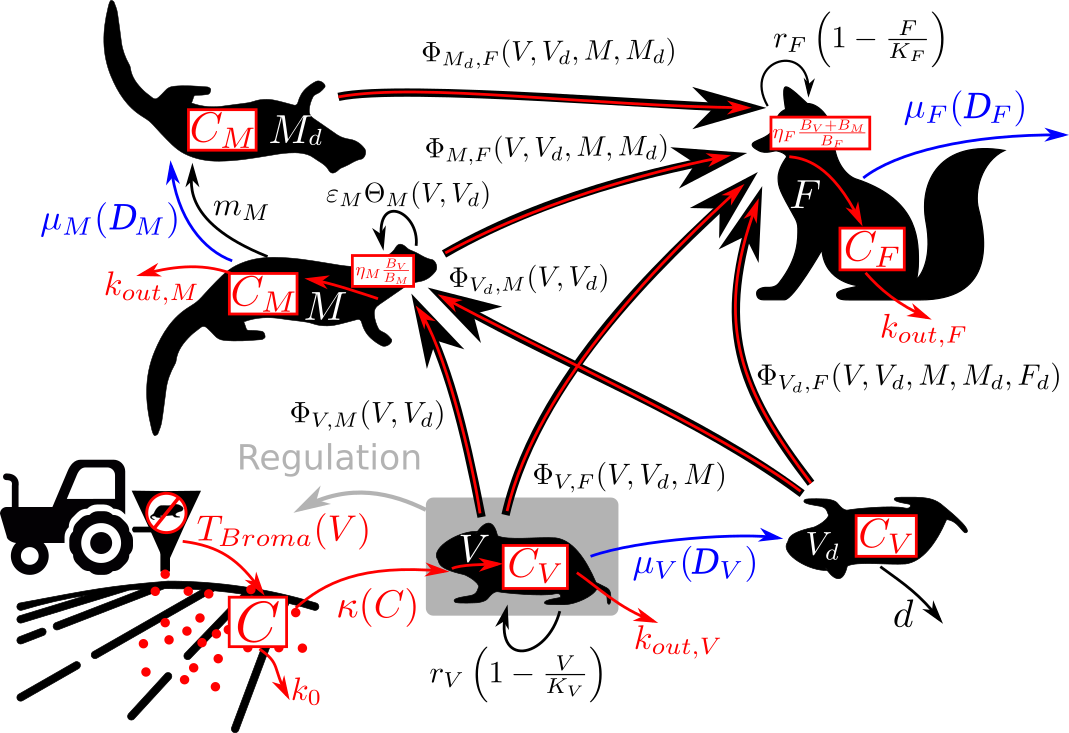
\includegraphics[width=.8\linewidth]{img/system_scheme.png}
		\caption{Flow diagram of the fate and impacts of anticoagulant rodenticide (AR, bromadiolone) in a tri-trophic food web. Black arrows and equations correspond to natural dynamics with trophic interactions, red arrows and equations represent the transfer of AR through the system and its accumulation into the different compartments. The arrows and equations in blue correspond to its impact (i.e., death of individuals) on the three species populations.}
		\label{fig:scheme}
	\end{center}
\end{figure}

% GRAPHIC POPULATION DYANMICS

\begin{figure}
	\begin{center}
		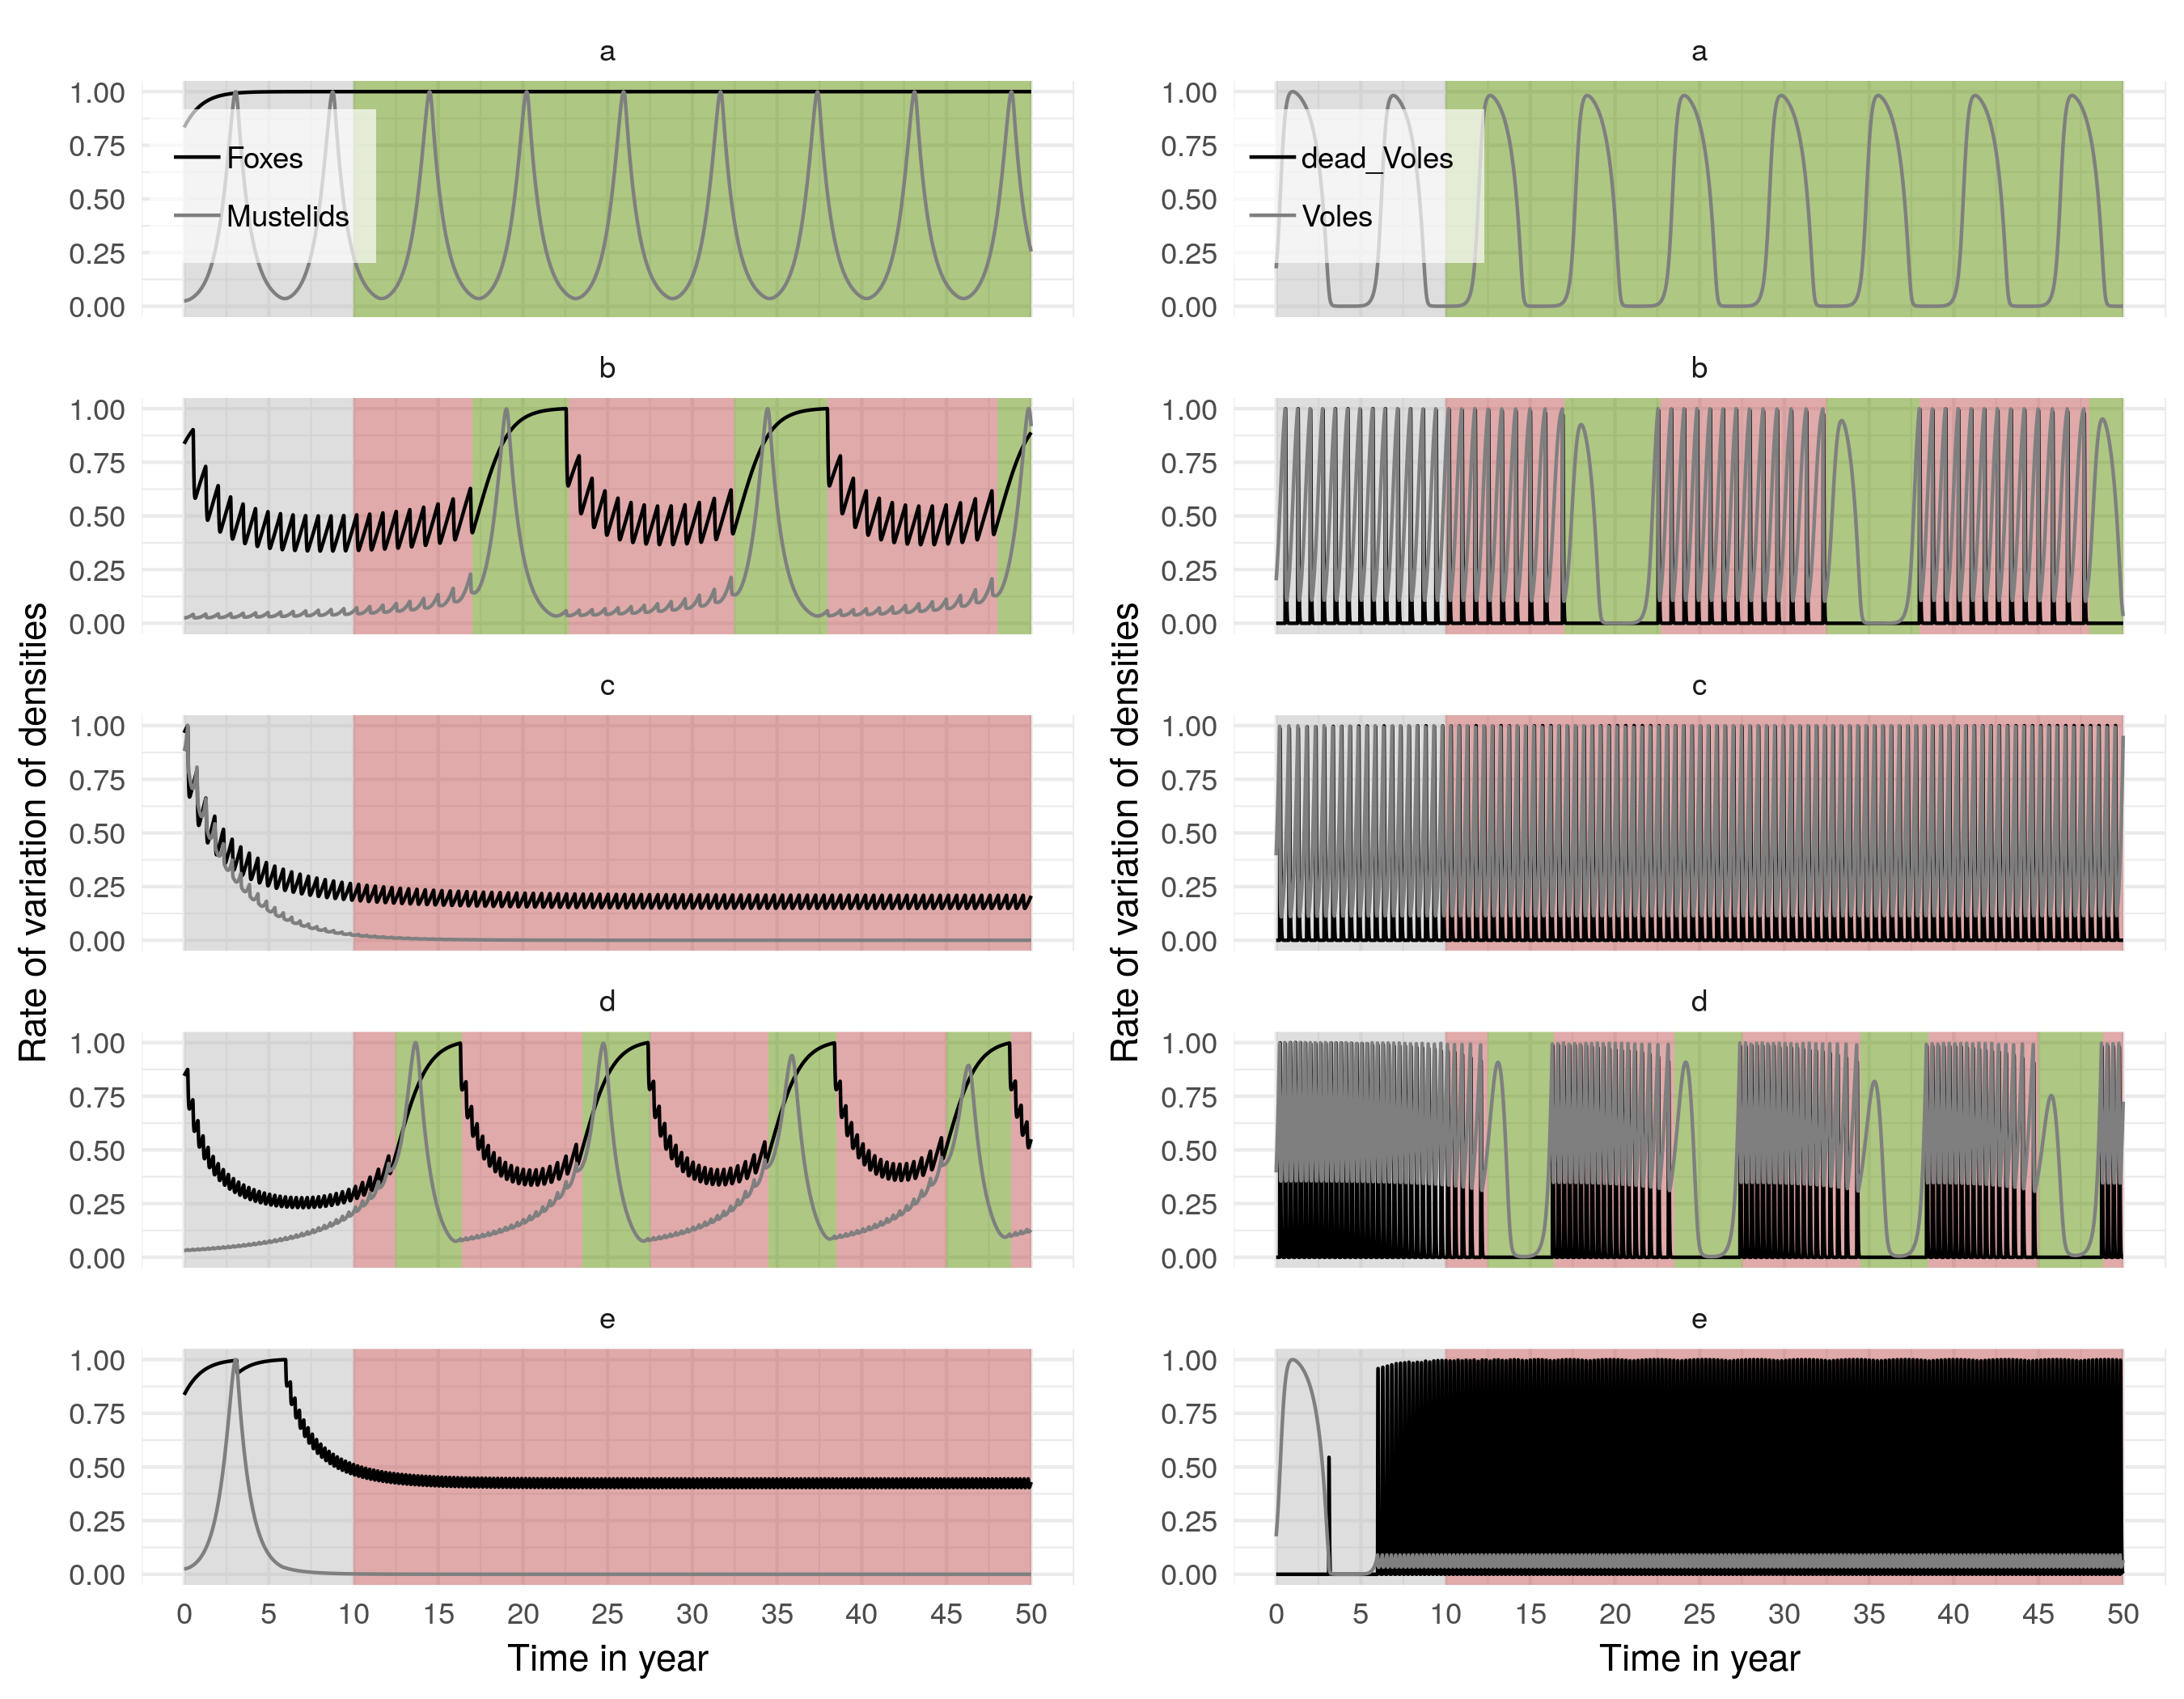
\includegraphics[width=\linewidth]{img/plot_join.png}
		\caption{Rate of variation of population densities simulated over 50 years (10 years of burn-in period in grey area): (Left) Dynamics of mustelids (grey line) and red foxes (black line), (Right) Dynamics of live (grey line) and dead (black line) voles. Letters at the top-center part of each sub-graph corresponds to the results obtained from each farmer functional response. Colored areas indicate the farmer-regulated (red area) and mustelid-regulated (blue area) periods of vole population dynamics respectively.}
		\label{fig:populations}
	\end{center}
\end{figure}

% GRAPHIC INTRAGUILD WITH AND WITHOUT FOXES

\begin{figure}
\begin{center}
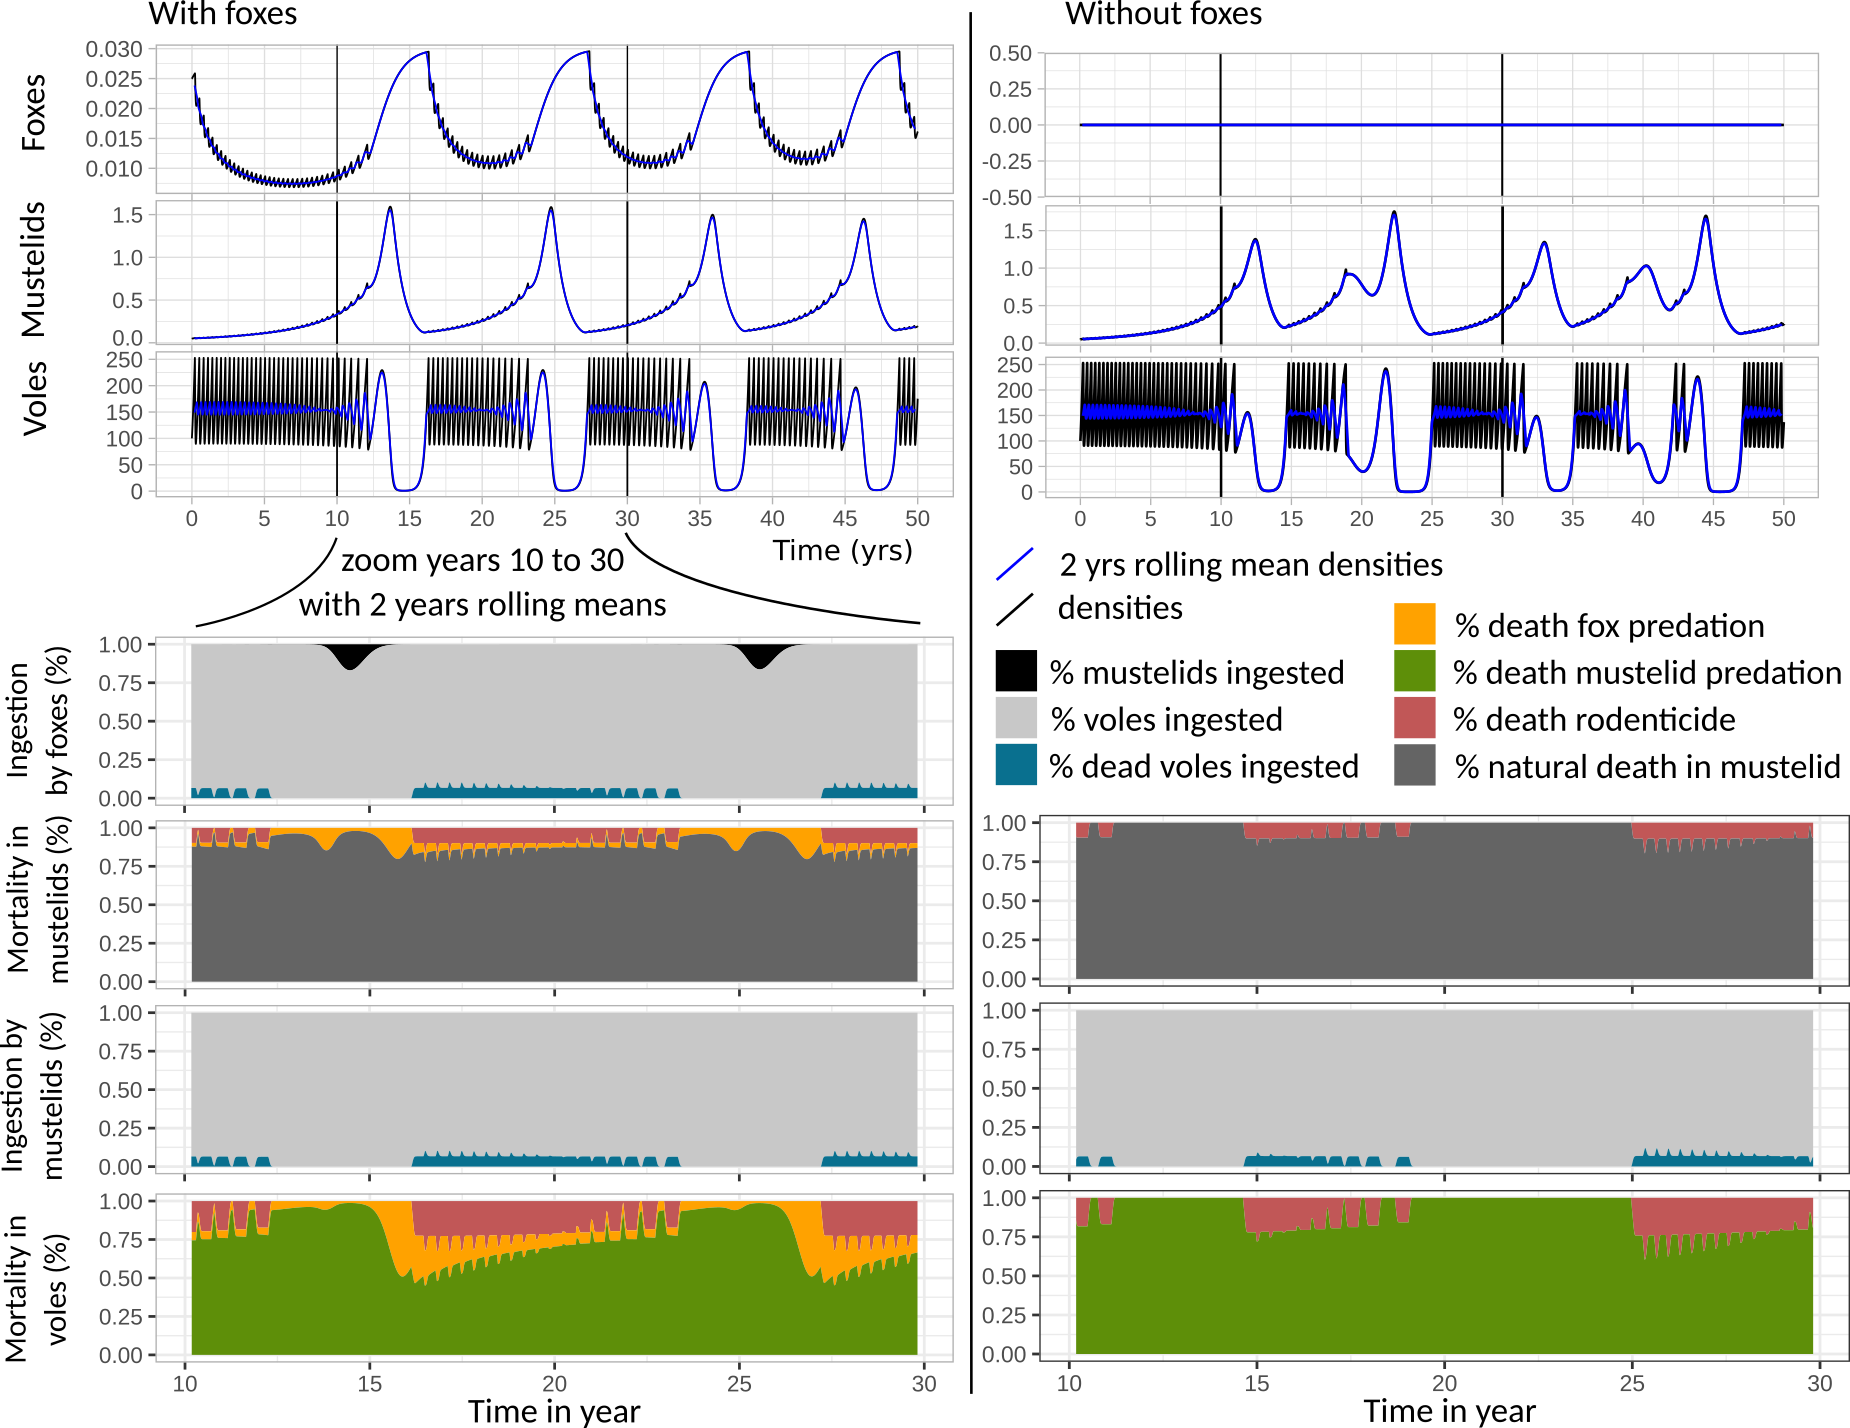
\includegraphics[width=\linewidth]{img/IGP_Graph.png}
\caption{Effects of intraguild predation. Top graphics: daily densities of voles (in black) and 2-years rolling means of densities (in blue) for the farmer functional response d (i.e., 7.5kg of rodenticide at threshold density of 250 voles) with and without foxes (left and right respectively). Bottom graphics: stacked charts of ingestion and mortality proportion.}
\label{fig:intraguild}
\end{center}
\end{figure}

% GRAPHIC SENSITIVITY ANALYSIS

\begin{figure}
	\begin{center}
		\includegraphics[width=\linewidth]{img/plt_sobolIndex_draw.jpg}
		\caption{First-order Sobol's sensitivity index (denoted $S_p$ for parameter $p$) providing the global sensitivity of cost functions to parameters of the model \citep{Sobol1993} for the model d (i.e., 7.5kg of AR at threshold density of 250 voles). Analysis is based on 4200 simulations. Values reflect the expected fractional reduction in the variance for each cost functions that would be achieved if a specific parameter is fixed. If $S_p = 1$, the sensitivity is not influenced by the parameter $p$.}
		\label{fig:sobol_sensitivity}
	\end{center}
\end{figure}


\end{document}
